% uid: ""
% school: "lycee"
% level: "1ere"
% chapter: "Théorème de Thalès et sa réciproque"
% title: "Deux segments égaux et un milieu"
% difficulty: "Moyen"
% tags: ["thales", "papillon", "triangle-isocele", "milieu"]
% provenance: "own"
% batch: "2026-11-22-revision-1ere-A"

% ---STATEMENT---
$ABC$ est un triangle isocèle en $A$. Le point $D$ est sur $[AB]$ et le point $E$ sur la demi-droite $[AC)$, au-delà de $C$, avec $BD=CE$. La droite $(DE)$ coupe $(BC)$ en $F$.
% alt: Triangle isocèle ABC, points D sur AB et E sur la demi-droite AC au-delà de C, droite DE coupant BC en F, parallèle à AC passant par D coupant BC en K
\begin{center}
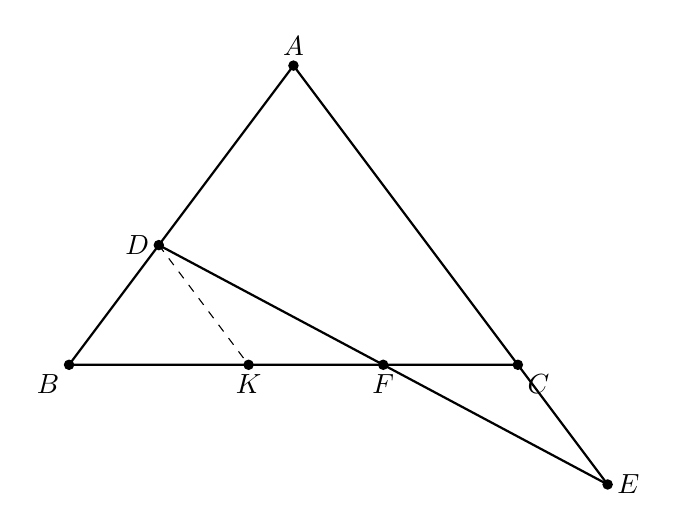
\begin{tikzpicture}[scale=0.95]
  \coordinate (B) at (0,0); \coordinate (C) at (6,0); \coordinate (A) at (3,4);
  \coordinate (D) at (1.2,1.6); \coordinate (E) at (7.2,-1.6); \coordinate (K) at (2.4,0); \coordinate (F) at (4.2,0);
  \draw[thick] (A)--(B)--(C); \draw[thick] (A)--(E); \draw[thick] (D)--(E); \draw[dashed] (D)--(K);
  \foreach \p/\pos in {A/above,B/below left,C/below right,D/left,E/right,K/below,F/below}{\fill (\p) circle (2pt) node[\pos]{$\p$};}
\end{tikzpicture}
\end{center}
\begin{enumerate}
  \item La parallèle à $(AC)$ passant par $D$ coupe $[BC]$ en $K$. Montrer que $DK=BD$.
  \item Montrer que $F$ est le milieu de $[DE]$. [Papillon de sommet $F$.]
  \item Application : $AB=AC=5$, $BC=6$ et $BD=2$. Calculer $BK$, puis $BF$.
  \item On pose $BD=t\,AB$ avec $0<t<1$. Montrer que $BF=\dfrac{1+t}2\,BC$. Où se trouve $F$ lorsque $D$ décrit $[AB]$ ?
  \item Avec les données de la question 3, pour quelle valeur de $BD$ a-t-on $BF=5$ ?
\end{enumerate}

% ---SOLUTION---
\begin{prop}[Thalès : triangle et papillon]
\textbf{Triangle.} $D\in[BA]$, $K\in[BC]$, $(DK)\parallel(AC)$ : on part de $B$, \ib{$\dfrac{BD}{BA}=\dfrac{BK}{BC}=\dfrac{DK}{AC}$}.

\textbf{Papillon.} Deux droites se coupent en $F$, avec $(DK)\parallel(EC)$ : on part de $F$, \ib{$\dfrac{FD}{FE}=\dfrac{FK}{FC}=\dfrac{DK}{EC}$}.
\end{prop}
\begin{enumerate}
  \item Dans le triangle $BAC$, on a $D\in[BA]$, $K\in[BC]$ et $(DK)\parallel(AC)$. Thalès de sommet $B$ :
  \[\dfrac{BD}{BA}=\dfrac{BK}{BC}=\dfrac{DK}{AC}\]
  On retient $\dfrac{DK}{AC}=\dfrac{BD}{BA}$, donc $DK=AC\times\dfrac{BD}{BA}$.

  Le triangle est isocèle en $A$ : $AC=BA$. Donc
  \[DK=\ib{$BD$}\]

  \item Les droites $(DE)$ et $(KC)=(BC)$ se coupent en $F$ ; les droites $(DK)$ et $(EC)=(AC)$ sont parallèles. Triangles $FDK$ et $FEC$ de sommet $F$ :
  \[\dfrac{FD}{FE}=\dfrac{FK}{FC}=\dfrac{DK}{EC}\]
  On a $DK=BD$ (question 1) et $BD=CE$ (hypothèse), donc $\dfrac{DK}{EC}=1$.

  Alors $FD=FE$ et $FK=FC$ :
  \[\ib{$F$ est le milieu de $[DE]$}\]
  et aussi le milieu de $[KC]$.

  \item Thalès de sommet $B$ avec $BD=2$ et $BA=5$ :
  \[\dfrac{BK}{BC}=\dfrac{BD}{BA}=\dfrac25\implies BK=\dfrac25\times6=\ib{$2{,}4$}\]
  Alors $KC=BC-BK=6-2{,}4=3{,}6$. $F$ est le milieu de $[KC]$ :
  \[KF=\dfrac{3{,}6}2=1{,}8\qquad BF=BK+KF=2{,}4+1{,}8=\ib{$4{,}2$}\]

  \item Thalès de sommet $B$ : $\dfrac{BK}{BC}=\dfrac{BD}{BA}=t$, donc $BK=t\,BC$ et $KC=(1-t)\,BC$.

  $F$ est le milieu de $[KC]$ :
  \[BF=BK+\dfrac{KC}2=t\,BC+\dfrac{1-t}2\,BC=\ib{$\dfrac{1+t}2\,BC$}\]
  Pour $0<t<1$, $BF$ est compris entre $\dfrac{BC}2$ et $BC$ : le point $F$ décrit le segment ouvert entre le milieu de $[BC]$ et $C$.

  \item Avec $BC=6$ : $BF=3\,(1+t)$.
  \[3\,(1+t)=5\iff1+t=\dfrac53\iff t=\dfrac23\]
  \[BD=t\times AB=\dfrac23\times5=\ib{$\dfrac{10}3$}\approx3{,}3\]
\end{enumerate}
\textbf{Idée :} la parallèle à $(AC)$ menée par $D$ déplace le segment $[BD]$ sans changer sa longueur (triangle isocèle $BDK$), ce qui fabrique un papillon de rapport $1$.

\textbf{Piège :} oublier que $AB=AC$ : sans cette hypothèse, $DK\neq BD$ et $F$ n'est plus le milieu.
